\documentclass{beamer}

\usepackage{proof}
\usepackage{cancel}
\usepackage{chronology}
\usepackage{graphicx}
\usepackage{ulem}
\usepackage{amsmath}
\usepackage{amssymb}
\usepackage{color}
%\usepackage{pstricks}
\setbeamertemplate{navigation symbols}{}

\renewcommand{\em}{\itshape}

\mode<presentation>
{
  \usecolortheme{crane}
  \usetheme{Frankfurt}
}
% \mode<presentation>
% {
%   \usecolortheme{dove}
% }

% \mode<presentation>
% {
% \useinnertheme[shadow=true]{rounded}
% \useoutertheme{infolines}
% \usecolortheme{dove}
% \setbeamerfont{block title}{size={}}
% }

\title[OBDA]{Ontology-based data access}

\author{Robert Hoehndorf}

\institute[KAUST]
{\includegraphics[width=.1\textwidth]{kaust_logo3.png}\\
  King Abdullah University of Science and Technology}

\date{}

\begin{document}
\begin{frame}
  \titlepage
\end{frame}

\begin{frame}
  \frametitle{Ontology-based data access}
  \begin{block}{}
    What do we gain when using ontologies to access our data?
  \end{block}
\end{frame}

\begin{frame}
  \frametitle{Ontology-based data access}
  \framesubtitle{Identify inconsistencies and incoherent descriptions of data}
  \begin{itemize}
    {\tiny
  \item {\tt 'prokaryotic cell' DisjointFrom: 'eukaryotic cell'}
  \item {\tt 'fungal cell' SubclassOf: 'eukaryotic cell'}
  \item {\tiny {\tt $spore_1$ instanceOf: 'fungal cell'}}
  \item {\tiny {\tt $spore_1$ instanceOf: 'prokaryotic cell'}}
    \begin{itemize}
    \item knowledgebase becomes inconsistent
    \end{itemize}
    \pause
  \item {\tt spore SubclassOf: 'fungal cell'}
  \item {\tt spore SubclassOf: 'prokaryotic cell'}}
    \begin{itemize}
    \item {\tt spore} becomes unsatisfiable
    \end{itemize}
  \end{itemize}
\end{frame}

\begin{frame}
  \frametitle{Ontology-based data access} 
  \framesubtitle{Enrich possibly incomplete data with background
    knowledge}
  Retrieve all patients with {\em Tetralogy of Fallot}:
  \vspace{1cm}
  \begin{columns}[onlytextwidth]
    \begin{column}{.5\textwidth}
      \centerline{\includegraphics[width=1\textwidth]{tetralogy.png}}
    \end{column}
    \begin{column}{.5\textwidth}
      {\tiny
      \begin{itemize}
      \item {\tt P instanceOf has-symptom some 'overriding aorta'}
      \item {\tt P instanceOf has-symptom some 'ventricular septal defect'}
      \item {\tt P instanceOf has-symptom some 'pulmonic stenosis'}
      \item {\tt P instanceOf has-symptom some 'right ventricular hypertrophy'}
      \end{itemize}
}
    \end{column}
  \end{columns}
\end{frame}

\begin{frame}
  \frametitle{Ontology-based data access} 
  \framesubtitle{Enrich the data schema used to query data sources
    with additional information}
  Retrieve all patients with {\em ventricular septal defect}:
  \vspace{1cm}
  \begin{columns}[onlytextwidth]
    \begin{column}{.5\textwidth}
      \centerline{\includegraphics[width=1\textwidth]{tetralogy.png}}
    \end{column}
    \begin{column}{.5\textwidth}
      {\tiny
      \begin{itemize}
      \item {\tt P instanceOf has-symptom some 'ICD9:745.2 (tetralogy of fallot)'}
      \end{itemize}
    }
    \end{column}
  \end{columns}
\end{frame}

\begin{frame}
  \frametitle{Ontology-based data access}
  \framesubtitle{Provide a uniform view over multi-modal data sources}
  \centerline{\includegraphics[width=1\textwidth]{fallot-slide.pdf}}
\end{frame}

\begin{frame}
  \setbeamercovered{transparent}
  \frametitle{The ontology-based data access paradigm}
  \begin{itemize}
  \item<1,2> Conceptual layer
    \begin{itemize}
    \item conceptual model
    \item domain model/ontologies
    \end{itemize}
  \item<1> Data layer
    \begin{itemize}
    \item single or federated {\em structured databases}
    \item text
    \item images
    \item custom files (sequences, genetic variation)
    \end{itemize}
  \item<1> Mapping between both
    \begin{itemize}
    \item explicit facts in a knowledge base
    \item direct, manual assertions/annotations
    \item concept recognition, entity recognition
    \item image processing
    \end{itemize}
  \end{itemize}
\end{frame}

\begin{frame}
  \frametitle{Ontology-based data access}
  \framesubtitle{Challenges for ontology-based access to biological data}
  \begin{itemize}
  \item hundreds of ontologies
  \item millions of classes
  \item complex/expressive ontologies
  \end{itemize}
  \centerline{\includegraphics[width=.6\textwidth]{bioportal-statistics.png}}
\end{frame}

\begin{frame}
  \frametitle{Web Ontology Language}
  \begin{itemize}
  \item based on Description Logic {\em SROIQ}
  \item satisfiability is decidable $\Rightarrow$ automated reasoning
  \item complexity for satisfiability in SROIQ is 2-NEXPTIME-complete
  \end{itemize}
  \centerline{\includegraphics[width=0.8\textwidth]{classifying.png}}
\end{frame}

\begin{frame}
  \frametitle{Modularization}
  \begin{itemize}
  \item tractable subsets of OWL 2: EL, QL, RL
  \item problem: given an OWL ontology $O$, can we identify a maximal
    (EL, QL, RL)-module of $O$?
  \end{itemize}
  \pause
  \begin{itemize}
  \item {\tt 'Abnormality of appendix' EquivalentTo: not (has-part some (Appendix
    and Normal))} ({\xcancel{EL}})
  \item {\tt 'Absent appendix' EquivalentTo: not (has-part some Appendix)} ({\xcancel{EL}})
  \end{itemize}
  \pause
  \begin{itemize}
  \item Inference: {\tt 'Absent appendix' SubclassOf: 'Abnormality of
      appendix'} (EL)
  \end{itemize}
\end{frame}

\begin{frame}
  \frametitle{Modularization}
  \begin{definition}
    Let $T$ be a set of $L_1$-formulas over $\Sigma$, and
    $L_2 \subseteq L_1$ a sub-language of $L_1$. The $L_2$-module of
    $T$ is defined as $T \cap Fm(L_2)$.
  \end{definition}
  \begin{itemize}
  \item Question: is the $EL$-module of a $SROIQ$-theory $T$ finitely
    axiomatizable?
  \item Given two sub-languages, $L_1$ and $L_2$, of FOL (e.g., OWL 2
    ($SROIQ$) and OWL 2 EL), $L_2 \subseteq L_1$, and a theory
    $T \subseteq Fm(L_1)$, can we find a finite set
    $Ax \subseteq Fm(L_2)$ such that
    $Ax^{\vdash_{L_2}} = T^{\vdash_{L_1}} \cap Fm(L_2)$?
  \end{itemize}

\end{frame}

\begin{frame}
  \frametitle{Modularization}
  \framesubtitle{EL Vira}
  \centerline{\includegraphics[width=0.5\textwidth]{elvira.png}}
  \url{http://el-vira.googlecode.com}
  \begin{itemize}
  \item ontology modularization 
  \item identify EL, QL, RL axiom patterns in the {\em deductive
      closure} of an ontology $\Rightarrow$ use of reasoner with full support of OWL
  \item retain signature of ontology
  \item maximality is open problem
    % \begin{itemize}
    % \item given $T_{SROIQ}$, identify $T_{EL}$
    %   s.t. ${T_{SROIQ}}^\vdash/_{EL} = {T_{EL}}^{\vdash_{EL}}$
    % \end{itemize}
  \end{itemize}
%  Hoehndorf et al., 2011
\end{frame}

\begin{frame}
  \frametitle{Modularization}
  \framesubtitle{EL Module}
  {\tiny
  \begin{itemize}
  \item \sout{{\tt 'Abnormality of appendix' EquivalentTo: not (has-part some (Appendix
    and Normal))}}
  \item \sout{{\tt 'Absent appendix' EquivalentTo: not (has-part some Appendix)}}
  \end{itemize}
  \begin{itemize}
  \item {\tt 'Absent appendix' SubclassOf: 'Abnormality of appendix'}
  \end{itemize}
}
\pause
\vspace{2cm}
Next: collect all the relevant ontologies in the domain
\end{frame}


\begin{frame}
  \frametitle{BioPortal}
  \centerline{\includegraphics[width=.9\textwidth]{bioportal-screen.png}}
\end{frame}

\begin{frame}
  \frametitle{BioPortal}
  \begin{itemize}
  \item SPARQL endpoint
  \item ontology recommender
  \item resource index
  \end{itemize}
\end{frame}

\begin{frame}
  \frametitle{OntoBee}
  \centerline{\includegraphics[width=.9\textwidth]{ontobee-screen.png}}\
\end{frame}

\begin{frame}
  \frametitle{Shortcomings}
  \begin{itemize}
  \item SPARQL endpoints: different semantics
  \item OWL reasoning not supported
  \end{itemize}
\end{frame}

\begin{frame}
  \frametitle{Aber-OWL Ontology Repository}
  \centerline{\url{http://aber-owl.net}}
  \vspace{1cm}
  \begin{itemize}
  \item contains a repository of biomedical ontologies (including all OBO ontologies)
  \item reasoning with the ELK reasoner
    \begin{itemize}
    \item OWL-EL
    \item parallel and incremental reasoning
    \end{itemize}
  \item web and JSON interface
  \item query single or multiple ontologies in the repository
  \item query ontologies on the web
  \end{itemize}
\end{frame}

\begin{frame}
  \frametitle{Aber-OWL Ontology Repository}
  \begin{quote}
    ``merely using ontologies [...] does not reduce heterogeneity: it
    just raises heterogeneity problems to a higher level''
  [Euzenat, 2007] \end{quote} 
  \begin{itemize}
  \item 471 ontologies
  \item 6,450,141 classes
  \item 67,786,617 logical axioms
  \item 3 inconsistent ontologies
  \item identifies many unsatisfiable classes
    \begin{itemize}
    \item even using only OWL EL!
    \item often due to changing imports
    \end{itemize}
  \end{itemize}
\end{frame}

\begin{frame}
  \frametitle{Aber-OWL Ontology Repository}
  Labels are not just {\tt rdfs:label}...
  \begin{itemize}
  \item Labels:
    \begin{itemize}
    \item {\tt rdfs:label}
    \item {\tt http://www.w3.org/2004/02/skos/core\#prefLabel}
    \item {\tt http://purl.obolibrary.org/obo/IAO\_0000111}
    \end{itemize}
  \item Defintions:
    \begin{itemize}
    \item {\tt http://www.w3.org/2004/02/skos/core\#definition}
    \item {\tt http://purl.org/dc/elements/1.1/description}
    \item {\tt
        http://www.geneontology.org/formats/\-oboInOwl\#hasDefinition}
    \item ...
    \end{itemize}
  \end{itemize}
\end{frame}

\begin{frame}
  \frametitle{Average query times}
  \begin{itemize}
  \item 10ms for a simple query (named classes)
  \item 240ms for query of complex concept descriptions
  \end{itemize}
\end{frame}

\begin{frame}
  \frametitle{Ontologies and graphs}
  \centerline{\includegraphics[width=.9\textwidth]{sio.png}}
\end{frame}

\begin{frame}
  \setbeamercovered{transparent}
  \frametitle{The ontology-based data access paradigm}
  \begin{itemize}
  \item<1> Conceptual layer
    \begin{itemize}
    \item conceptual model
    \item domain model/ontologies
    \end{itemize}
  \item<2> Data layer
    \begin{itemize}
    \item single or federated {\em structured databases}
    \item text
    \item images
    \item custom files (sequences, genetic variation)
    \end{itemize}
  \item<3,4> Mapping between both
    \begin{itemize}
    \setbeamercovered{transparent}
    \item<3,4> explicit facts in a knowledge base
    \item<3,4> direct, manual assertions/annotations
    \item<3> concept recognition, entity recognition
    \item<3> image processing
    \end{itemize}
  \end{itemize}
\end{frame}

\begin{frame}[fragile]
  \frametitle{Aber-OWL: SPARQL}
  \centerline{\url{http://aber-owl.net/aber-owl/sparql/}}
  \vspace{1cm}
  Retrieve all proteins annotated to a part of apoptosis:
  {\tiny
\begin{verbatim}
PREFIX GO: <http://purl.uniprot.org/go/>
PREFIX taxon:<http://purl.uniprot.org/taxonomy/>
PREFIX up: <http://purl.uniprot.org/core/>
PREFIX skos: <http://www.w3.org/2004/02/skos/core#>

SELECT DISTINCT ?pname ?protein ?label ?ontid WHERE { 
  VALUES ?ontid { 
    OWL subclass <http://aber-owl.net/aber-owl/service/> <>
      { part_of some 'apoptotic process' }
  } . 
  ?protein a up:Protein .
  ?protein up:organism taxon:9606 .
  ?protein up:mnemonic ?pname .
  ?protein up:classifiedWith ?ontid .
  ?ontid skos:prefLabel ?label .
}
\end{verbatim}
}
\end{frame}

\begin{frame}[fragile]
  \frametitle{Aber-OWL: SPARQL}
  \centerline{\url{http://aber-owl.net/aber-owl/sparql/}}
  \vspace{1cm}
  Retrieve all proteins annotated to a part of apoptosis:
  {\tiny
\begin{verbatim}
PREFIX GO: <http://purl.uniprot.org/go/>
PREFIX taxon:<http://purl.uniprot.org/taxonomy/>
PREFIX up: <http://purl.uniprot.org/core/>
PREFIX skos: <http://www.w3.org/2004/02/skos/core#>

SELECT DISTINCT ?pname ?protein ?label ?ontid WHERE { 
  VALUES ?ontid { 
    GO:0071550 GO:0006309 GO:0042771 GO:0070059 GO:0039650 GO:0043154
    GO:0097345 GO:0097297 GO:0008637 GO:0001836 GO:1902109 ...
  } . 
  ?protein a up:Protein .
  ?protein up:organism taxon:9606 .
  ?protein up:mnemonic ?pname .
  ?protein up:classifiedWith ?ontid .
  ?ontid skos:prefLabel ?label .
}
\end{verbatim}
}
\end{frame}

\begin{frame}
  \frametitle{Aber-OWL: SPARQL}
  \centerline{\includegraphics[width=1.1\textwidth]{uniprot-aber.png}}
\end{frame}

\begin{frame}
  \frametitle{Aber-OWL: SPARQL}
  \begin{itemize}
  \item SPARQL query expansion
  \item integration of DL queries in SPARQL
  \item one problem: IRIs difference between SPARQL endpoints
  \end{itemize}
\end{frame}

\begin{frame}
  \setbeamercovered{transparent}
  \frametitle{The ontology-based data access paradigm}
  \begin{itemize}
  \item<0> Conceptual layer
    \begin{itemize}
    \item conceptual model
    \item domain model/ontologies
    \end{itemize}
  \item<0> Data layer
    \begin{itemize}
    \item single or federated {\em structured databases}
    \item text
    \item images
    \item custom files (sequences, genetic variation)
    \end{itemize}
  \item<1,2> Mapping between both
    \begin{itemize}
    \item<1> explicit facts in a knowledge base
    \item<1> direct, manual assertions/annotations
    \item<2> concept recognition, entity recognition
    \item<0> image processing
    \end{itemize}
  \end{itemize}
\end{frame}

\begin{frame}
  \frametitle{Aber-OWL: Pubmed}
  \framesubtitle{Concept recognition}
  \begin{itemize}
  \item find mentions of ontology classes in text
  \item common approaches:
    \begin{itemize}
    \item use labels and synonyms
    \item stemming, text segmentation, POS tagging, machine learning
    \end{itemize}
  \end{itemize}
\end{frame}

\begin{frame}
  \frametitle{Aber-OWL: Pubmed}
  Aber-OWL: PubMed: 
  \begin{itemize}
  \item Lucene index of Medline and PubMed Central
  \item identify labels and synonyms of class {\em and subclasses}
  \item stop words, stemming, case removal
  \item combine text mining and reasoning over ontologies: find
    mentions of classes satisfying an OWL queries
  \item ``lightweight'' concept recognition, but high speed over
    large volumes of text (query time $<100ms$)
  \end{itemize}
\end{frame}

\begin{frame}
  \frametitle{Aber-OWL: PubMed}
  \framesubtitle{Retrieve documents mentioning 'ventricular septal defect'}
  \centerline{\includegraphics[width=1\textwidth]{aber-pubmed-search.png}}
\end{frame}

\begin{frame}
  \frametitle{Aber-OWL: PubMed}
  \begin{itemize}
  \item concept recognition incorporates automated reasoning (ontology
    hierarchy, axiom patterns)
  \item recognition of complex concepts (class expressions)
  \item useful for difficult concepts (gene functions, processes,
    phenotypes)
  \end{itemize}
\end{frame}

\begin{frame}
  \frametitle{Aber-OWL: PubMed}
  \centerline{http://aber-owl.net/aber-owl/diseasephenotypes/}
  \begin{itemize}
  \item find phenotypes (signs and symptoms) associated with common
    diseases
    \begin{itemize}
    \item no resource available for comparison
    \end{itemize}
  \item pattern-based mining of literature with Aber-OWL: PubMed
  \item evaluation (of genetically based disease phenotypes) with
    experimentally validated disease genes
  \end{itemize}
\end{frame}

\begin{frame}
  \frametitle{Aber-OWL: PubMed}
  \framesubtitle{http://aber-owl.net/aber-owl/diseasephenotypes/}
  \centerline{\includegraphics[width=1\textwidth]{aber-owl-plague.png}}
\end{frame}

\begin{frame}
  \frametitle{Aber-OWL: PubMed}
  \framesubtitle{http://aber-owl.net/aber-owl/diseasephenotypes/}
  \centerline{\includegraphics[width=1\textwidth]{pmi-auc-plot.pdf}}
\end{frame}

\begin{frame}
  \frametitle{Aber-OWL: PubMed}
  \centerline{\includegraphics[width=.9\textwidth]{network.eps}}
\end{frame}

\begin{frame}
  \frametitle{Diseases and phenotypes}
  \begin{block}{Phenotypes}
    Phenotypes are the observable characteristics of an organism arising
    from its {\em genotype} and its response to the {\em environment}.
  \end{block}
  \vspace{1cm}
  
  Analysis of phenotypes should reveal information about
  \begin{itemize}
  \item genotype,
  \item environment,
  \item mechanisms and processes that determine phenotype from genotype.
  \end{itemize}
\end{frame}

\begin{frame}
\frametitle{Phenotypes}
\framesubtitle{In biodiversity and ecology}
\centerline{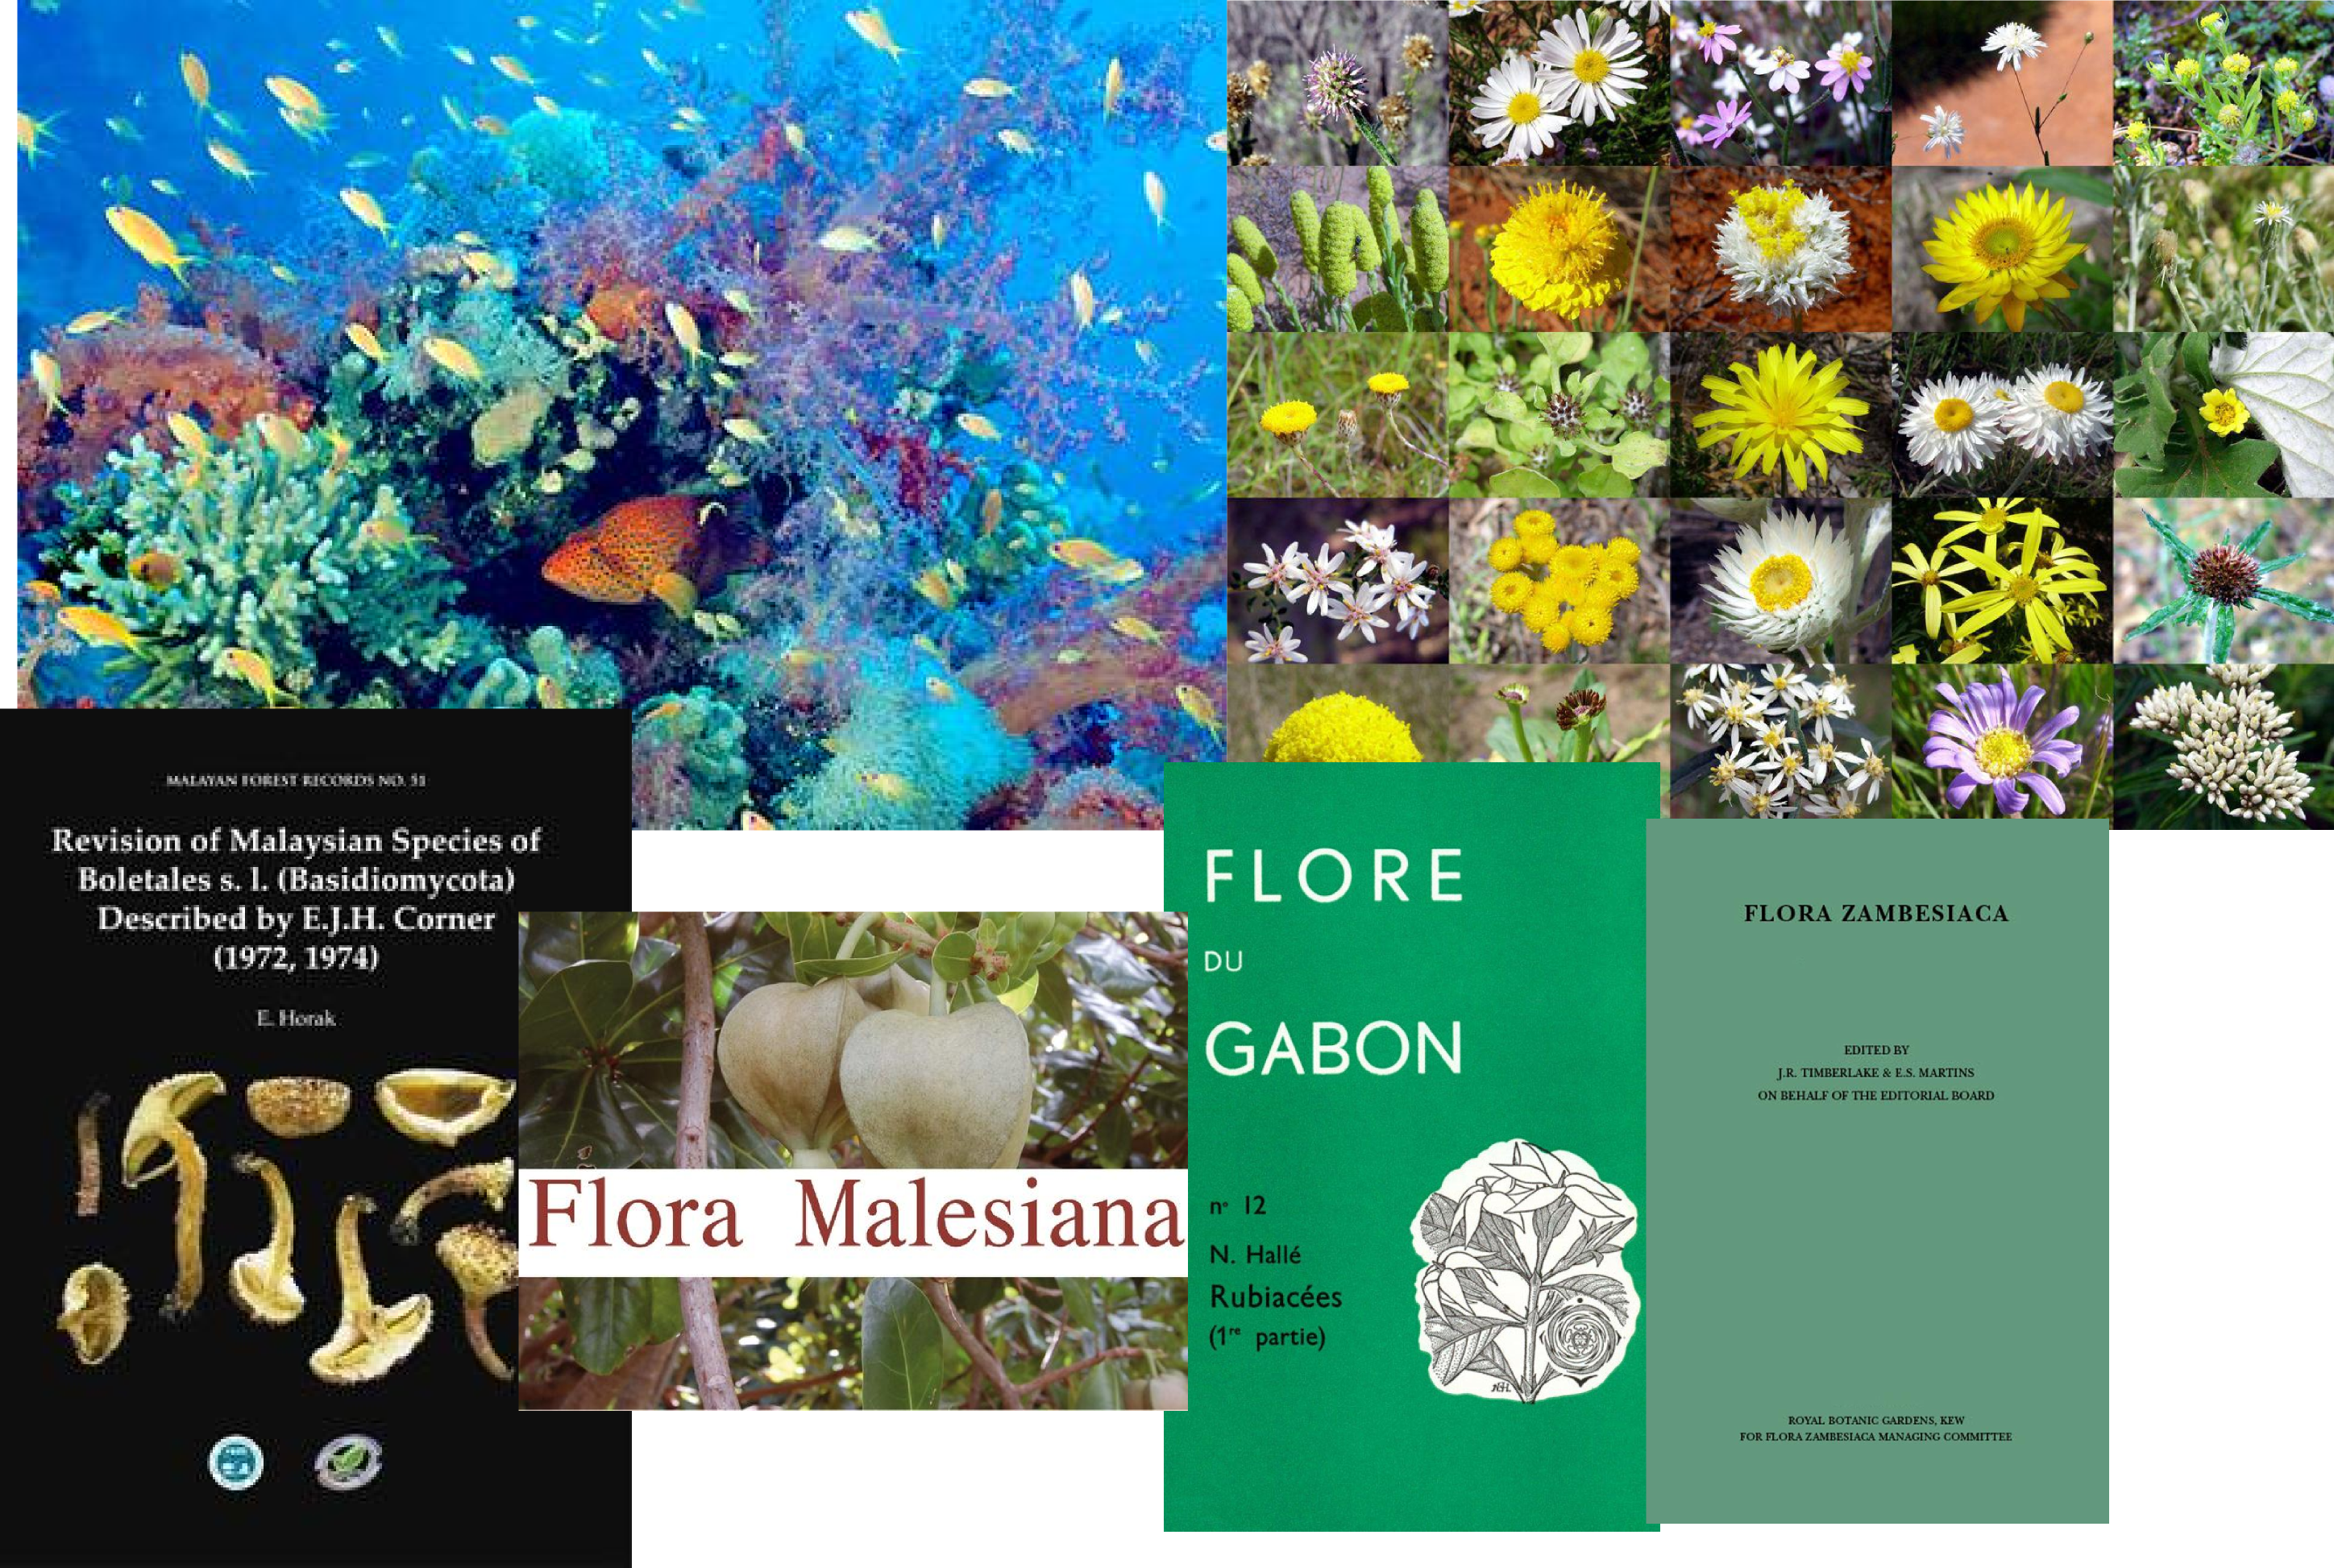
\includegraphics[width=\textwidth]{biodiv.png}}
\end{frame}

\begin{frame}
\frametitle{Phenotypes}
\framesubtitle{In evolutionary biology}
\centerline{\includegraphics[width=.8\textwidth]{phylogen.png}}
\end{frame}

\begin{frame}
\frametitle{Phenotypes}
\framesubtitle{In the clinic}
\centerline{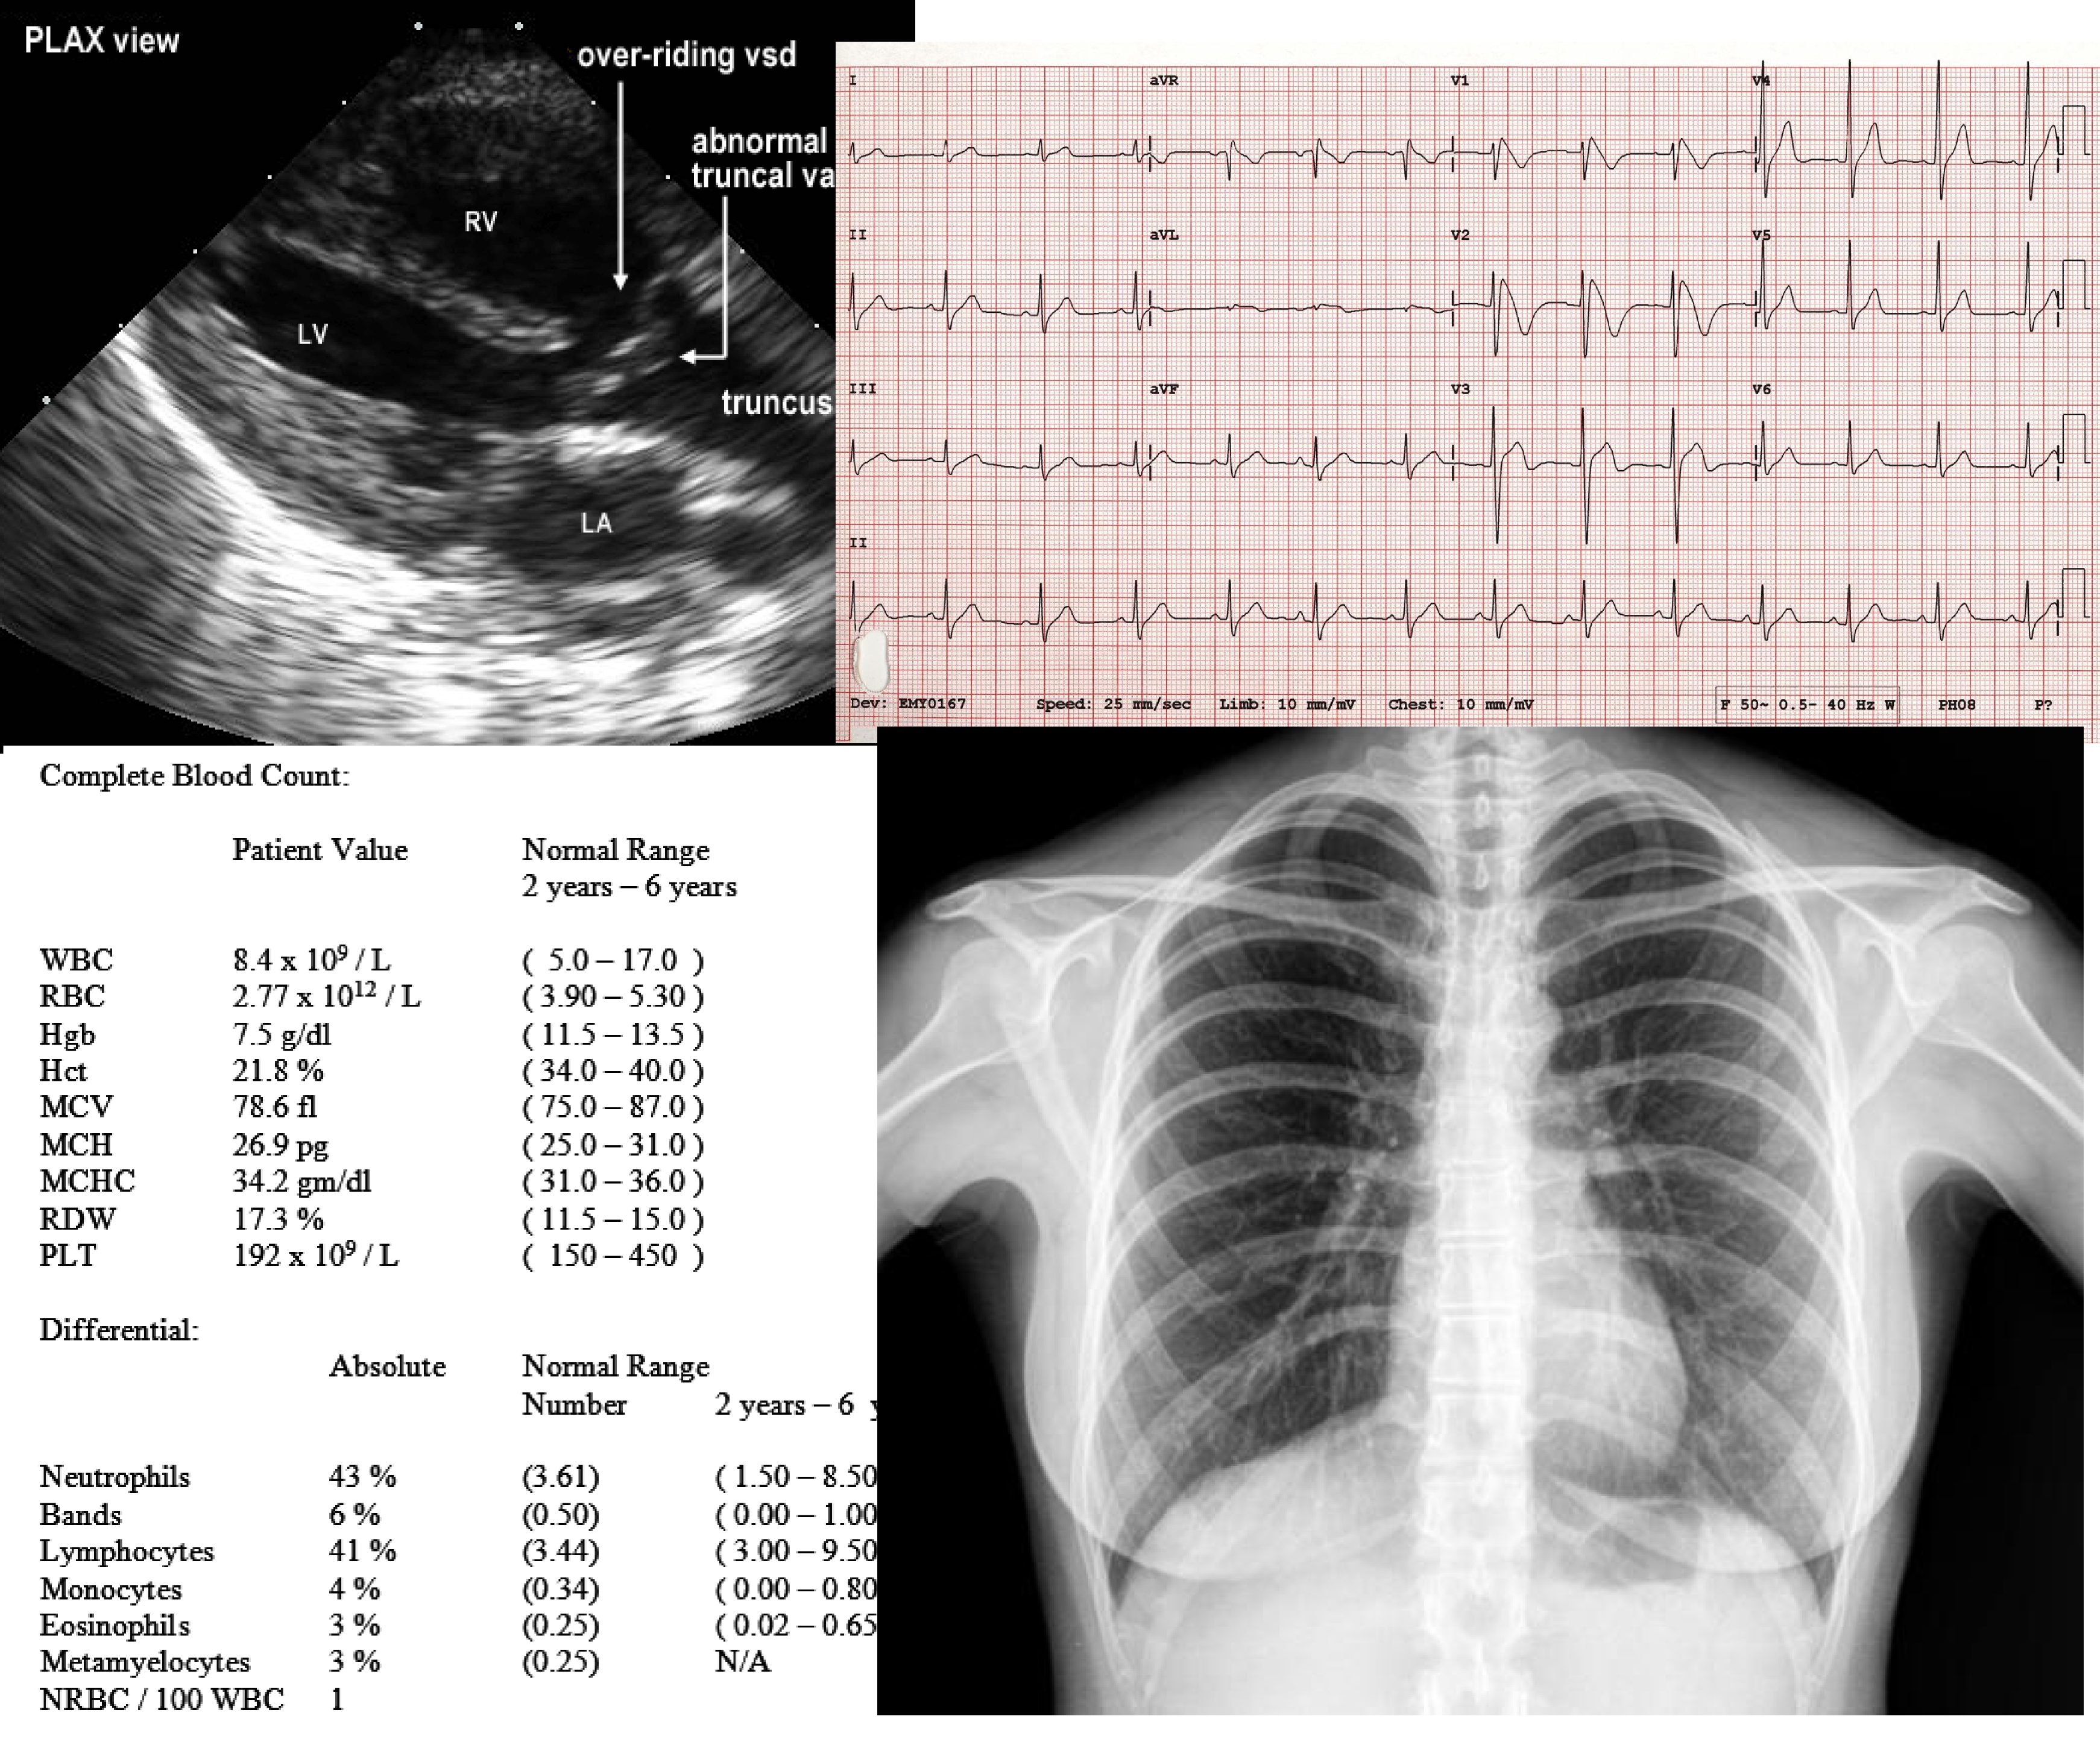
\includegraphics[width=1\textwidth]{clinic.png}}

\end{frame}

\begin{frame}
\frametitle{Phenotypes}
\framesubtitle{In the lab}
\centerline{\includegraphics[width=.8\textwidth]{lab.png}}
\end{frame}

\begin{frame}
\frametitle{Phenotypes}
\framesubtitle{Approach}
We want to:
\begin{enumerate}
\item describe phenotypes formally
  \begin{itemize}
  \item morphology
  \item function
  \item $\Rightarrow$ formal ontology
  \end{itemize}
  \pause
\item integrate/compare phenotypes (within and between species)
  \begin{itemize}
  \item homologous organ structures
  \item related/identical function
  \item $\Rightarrow$ ontologies and automated reasoning
  \end{itemize}
  \pause
\item understand genotype-phenotype relations
  \begin{itemize}
  \item use morphological or functional similarity
  \item similarity in attribute values
  \item $\Rightarrow$ semantic similarity
  \end{itemize}
\end{enumerate}
\end{frame}

\begin{frame}
\frametitle{Phenotype representation}
\framesubtitle{EQ formalism}
\begin{block}{Entity + Quality = Phenotype}
A phenotype can be described by an entity and its quality.
\end{block}
\pause

\centerline{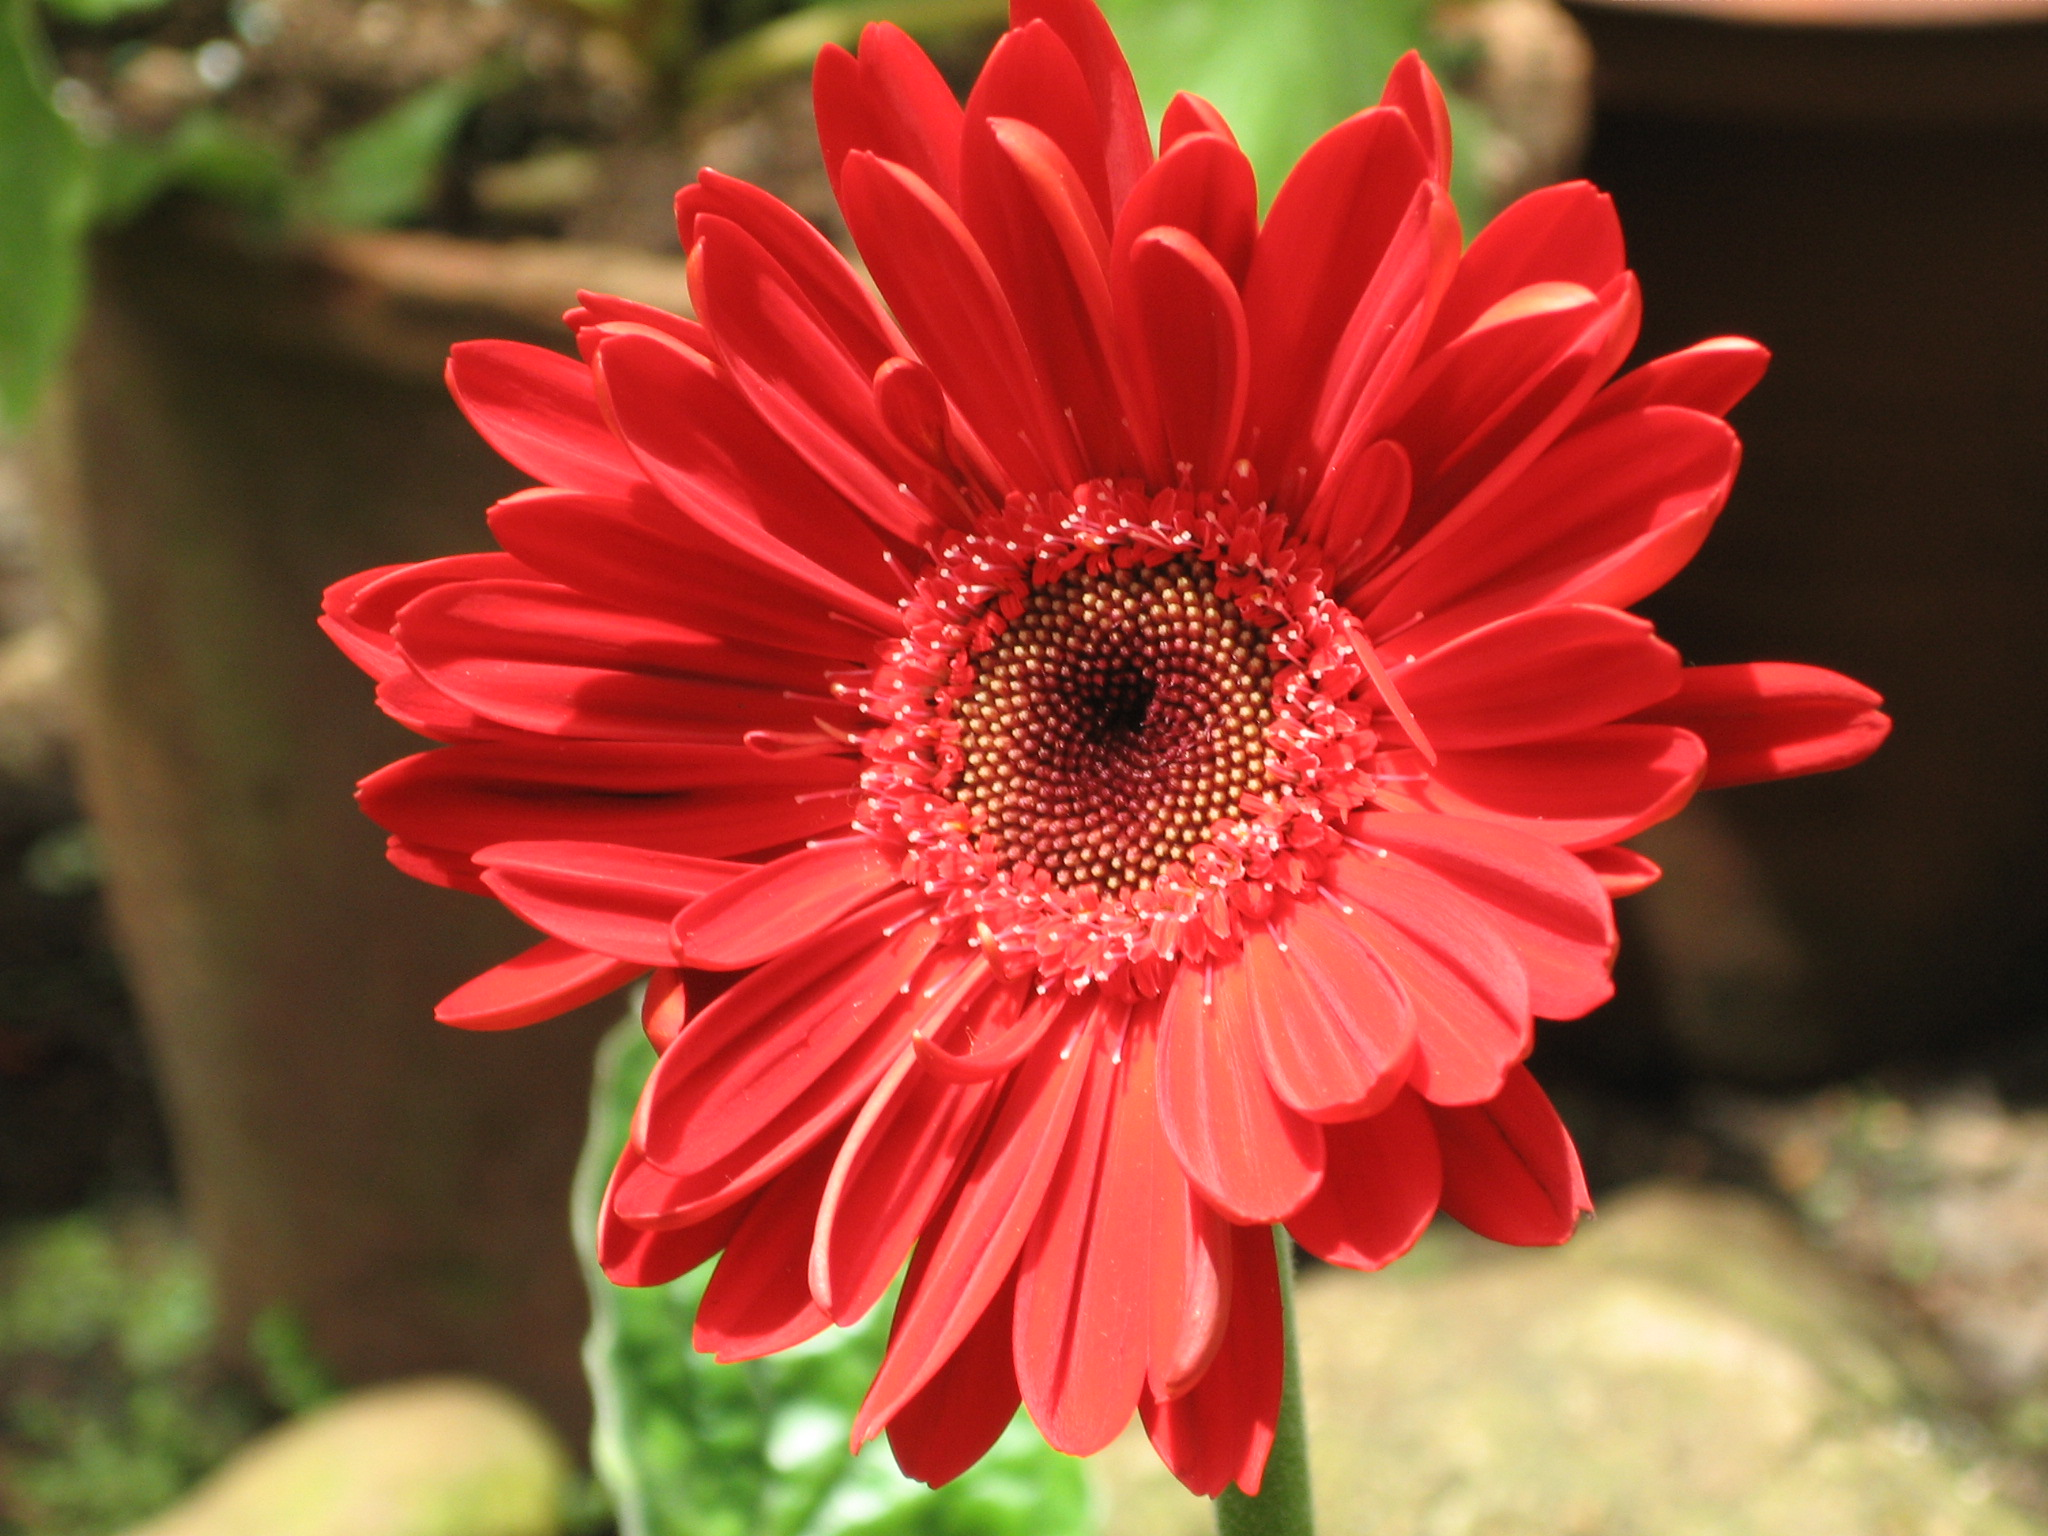
\includegraphics[width=.5\textwidth]{red-flower.png}}

Flower: red\\
\pause
Flower: {\tt PO:0009046} (Plant Ontology)\\
\pause
Red: {\tt PATO:0000322} (Phenotype And Trait Ontology)
\end{frame}

\begin{frame}
\frametitle{Phenotype representation}
\framesubtitle{EQ formalism}
\begin{block}{Entity 1 + Quality +Entity 2 = Phenotype}
Some qualities involve a second entity.
\end{block}

\centerline{\includegraphics[width=.5\textwidth]{Plant_response_to_stimuli.png}}

\pause
Leaf: {\tt PO:0025034} (Plant Ontology)\\
\pause
responsive to: {\tt PATO:0000487} (Phenotype And Trait Ontology)\\
\pause
detection of mechanical stimulus: {\tt GO:0050982} (Gene Ontology)
\end{frame}

\begin{frame}
\frametitle{Phenotype representation}
\framesubtitle{EQ formalism}
Entity + Quality = Phenotype

Entity 1 + Quality + Entity 2 = Phenotype
\begin{itemize}
\item Entity from reference ontology (Gene Ontology, anatomy ontology)
\item Quality from PATO ontology
%\item Quality {\bf inheres in} Entity
\end{itemize}
\end{frame}

\begin{frame}
  \frametitle{Phenotype representation}
  A phenotype is a quality that inheres in its bearer [Mungall, 2010].
  \begin{itemize}
  \item Red flower:
    $Red(x) \land \exists y ( inheresIn(x,y) \land Flower(y))$
  \item $Red \sqcap \exists inheresIn.Flower$
  \item Red: reuse an ontology of qualities
  \item Flower: reuse ontology of plant anatomy
  \end{itemize}
\end{frame}

\begin{frame}
\frametitle{Phenotype representation}
\framesubtitle{EQ formalism: semantics}
  Absent tail:
  \begin{itemize}
  \item $AbsentTail \equiv Absent \sqcap \exists inheresIn.Tail$
    \pause
  \item $AbsentTail \equiv LacksParts \sqcap \exists towards.Tail
    \sqcap \exists inheresIn.MouseBody$
    \pause
  \item $AbsentTail \equiv LacksParts \sqcap \exists towards.\{Tail\}
    \sqcap \exists inheresIn.MouseBody$ (Mungall, 2007)
    \pause
  \item no use of {\bf part-of} or {\bf has-part} relations
  \item no reuse of {\bf part-of} in anatomy ontology
    \pause
  \item Observation: having or lacking parts (functions, dispositions,
    processes, ...) are not {\em primarily} qualities.
  % \item $AbsentTail \sqsubseteq \neg \exists hasPart.Tail$ (H
  %   et al., 2007)
  %   \pause
  % \item $AbsentTail \sqsubseteq \exists pheneOf.(Organism \sqcap \neg
  %   \exists hasPart.Tail)$ (H et al., 2010)
  \end{itemize}
\end{frame}

\begin{frame}
  \frametitle{Phenotypic properties}
  \framesubtitle{Definition}
  A {\em phenotypic property} (phene) is the basic observable
  characteristic possessed by an organism.
  \begin{itemize}
  \item {\bf phene-of} and {\bf has-phene} relations
  \item examples: having weight, being red, not having an appendix as
    part, participating in mating behaviour
  \item based on a {\em defining class} $Y$
  \end{itemize}
  Definition pattern: \texttt{X EquivalentTo: pheneof some Y}
\end{frame}

\begin{frame}
\frametitle{Properties}
\framesubtitle{Taxonomy of properties}
Top-level ontology of properties based on defining class $Y$:
\begin{itemize}
\item Structural: having parts, lacking parts, being part of, not
  being part of
  \begin{itemize}
  \item $\exists pheneOf.(Mouse \sqcap \exists hasPart.Tail)$
  \end{itemize}
\item Qualitative: having qualities, lacking qualities, having
  quality-values, not having quality-values
  \begin{itemize}
  \item $\exists pheneOf.(Flower \sqcap \exists hasQuality.Red)$
  \end{itemize}
\item Functional: being capable to do $X$, not being capable to do
  $X$, being dysfunctional w.r.t. $F$
  \begin{itemize}
  \item $\exists pheneOf.(Heart \sqcap \exists hasFunction.PB)$
  \end{itemize}
\item Participatory: pumping blood, being a catalyst
  \begin{itemize}
  \item $\exists pheneOf.(Heart \sqcap \exists participatesIn.PB)$
  \end{itemize}
\end{itemize}
\end{frame}

\begin{frame}
\frametitle{Phenotype representation}
\begin{itemize}
\item {\tt phene-of} is functional:
  $\forall x,y,z (pheneOf(x,y) \land pheneOf(x,z) \rightarrow y=z)$
  \begin{itemize}
  \item alternatively: $\forall x,y(pheneOf(x,y) \rightarrow
    inheresIn(x,y))$, inherit functionality, NMP from GFO
  \end{itemize}
\item Absent tail:
  $AbsentTail \sqsubseteq \exists pheneOf.(Organism \sqcap \neg
  \exists hasPart.Tail)$
\item Dysfunctional heart: $DH \sqsubseteq \exists pheneOf.(Heart
  \sqcap \neg \exists hasFunction.PumpingBlood)$
\end{itemize}
\end{frame}

\begin{frame}
  \frametitle{Absence}
  \framesubtitle{Absent tail}
  \begin{figure}
    \includegraphics[scale=.5]{incon.pdf}
  \end{figure}
  \begin{itemize}
  \item $AbsentTail \sqsubseteq \exists pheneOf.(Mouse \sqcap \neg
    \exists hasPart.Tail)$
  \item MA: $Mouse \sqsubseteq \exists hasPart.Tail$
  \item $Mouse(Jerry), AbsentTail(x), hasPhene(Jerry, x)$
  \end{itemize}
%  \alert{Logical inconsistency!}
\end{frame}

\begin{frame}
  \frametitle{Absence}
  \framesubtitle{Absent appendix}
  \begin{itemize}
  \item Removal of conflicting axioms (has-part/part-of in anatomy)
    \pause
  \item Contextualize anatomy:
    \begin{itemize}
    \item $Normal \sqcap Mouse \sqsubseteq \exists hasPart.(Normal
      \sqcap Tail)$
    \item Needs one {\em Normal} for each axiom
    \end{itemize}
    \pause
  \item Rewrite anatomy using non-monotonic reasoning:
    \begin{itemize}
    \item {\em Normally:} $Mouse \sqsubseteq \exists hasPart.Tail$
    \item Circumscription of $\neg Normal$
    \item Better: use default logic and answer set programming
    \item $Mouse(x):hasPart(x,y)\land Tail(y)/hasPart(x,y)\land Tail(y)$
    \item Implementation in dlvhex 
    \item {\small \texttt{IC-has-part(X,Y) :-
          ind(X),class(Y),inst(X,Z), CC-normally-has-part(Z,Y), not
          IC-lacks-has-part(X,Y), class(Z).}}
    \end{itemize}
  \end{itemize}
\end{frame}

\begin{frame}
  \frametitle{Phenotype representation} 
  Ontologies can be used to {\em formally} 
  describe phenotypes and integrate phenotype descriptions with
  ontologies of anatomy and functions. We applied this method to
\begin{itemize}
\item Arabidopsis Information Resource
\item Gramene
\item WormBase
\item FlyBase
\item Saccharomyces Genome Database
\item Mouse Genome Informatics database
\item Zebrafish Model Organism Database
\item OMIM
\item OrphaNet
\item ...
\end{itemize}
\pause
... but all of them have different anatomy and physiology.
\end{frame}

\begin{frame}
  \frametitle{Crossspecies integration}
  \begin{center}
    Can we use this framework for data integration {\em across} species?
  \end{center}
  % \pause
  % \begin{center}
  %   Find all regions in the human {\em and mouse} genome sequences that are
  %   associated with Tetralogy of Fallot.
  % \end{center}
\end{frame}

\begin{frame}
  \frametitle{Crossspecies integration}
  \begin{itemize}
  \item UBERON ontology of homologous organ structures
    \begin{itemize}
    \item {\em Heart (human)} homologous to {\em Heart (mouse)}
    \pause
    \item {\em Tail (mouse)} homologous to... ?
      \pause
    \item {\em Tail (mouse)} SubClassOf: part-of some {\em Trunk
        (mouse)}
    \item {\em Trunk (mouse)} homologous to {\em Trunk (human)}
    \end{itemize}
    What if we treat homologous organ structures as {\em equivalent}
    (for this purpose)?
  \end{itemize}
\end{frame}

\begin{frame}
  \frametitle{Crossspecies integration}
  \begin{itemize}
  \item Human absent appendix: $\exists pheneOf.(Human \sqcap \neg
    \exists hasPart.HumanAppendix)$
  \item Mouse absent appendix: $\exists pheneOf.(Mouse \sqcap \neg
    \exists hasPart.MouseAppendix)$
  \item Mouse homologous to (equivalent to) Human
  \item MouseAppendix homologous to (equivalent to) HumanAppendix
  \item $\Rightarrow$ Human absent appendix equivalent to Mouse absent
    appendix
  \end{itemize}
\end{frame}

\begin{frame}
  \frametitle{Crossspecies integration}
  \begin{itemize}
  \item Mouse absent tail: $\exists pheneOf.(Mouse \sqcap \neg
    \exists hasPart.MouseTail)$
  \item MouseTail homologous to (equivalent to) ???
    \pause 
  \item Infer using mouse anatomy
  \end{itemize}
\end{frame}

\begin{frame}
  \frametitle{Crossspecies integration}
  Starting with a pair of Entity and Quality, generate the following classes:
  \begin{itemize}
  \item $EPhenotype \equiv \exists pheneOf.(\exists partOf.E \sqcap
    \exists hasQuality.\top)$
  \item 'E Q' $\equiv \exists pheneOf.(E \sqcap \exists hasQuality.Q)$
    \begin{itemize}
    \item or any of the other structural forms, depending on $Q$
    \end{itemize}
  \item assert equivalence between $E$s in different species (based on
    homology)
  \item then, include anatomy ontologies
    \pause
  \item AbsentTail (mouse) will become a subclass of TrunkPhenotype
    (mouse, human)
  \end{itemize}
\end{frame}

\begin{frame}
  \frametitle{Phenotype representation} 
\begin{itemize}
\item Arabidopsis Information Resource
\item Gramene
\item WormBase
\item FlyBase
\item Saccharomyces Genome Database
\item Mouse Genome Informatics database
\item Zebrafish Model Organism Database
\item OMIM
\item OrphaNet
\end{itemize}
\pause
\begin{itemize}
\item more than 250,000 formal phenotype descriptions
\item $>$ 2,000,000 axioms
\item $\Rightarrow$ Elvira modularization method
\end{itemize}
\end{frame}

\begin{frame}
  \frametitle{Crossspecies integration}
  \begin{itemize}
  \item Classify the resulting ontology using a OWL (EL) reasoner
    \pause 
  \item 70\% of classes are unsatisfiable... why?
    \pause
  \item it's not so easy to combine different anatomy ontologies;
    different conceptualizations!
    \begin{itemize}
    \item Anus (human) is an orifice which is a kind of {\em
        immaterial anatomical entity}; Anus (mouse) is a {\em material
        entity}
    \item {\em immaterial anatomical entity} and {\em material
        anatomical entity} are disjoint in human anatomy
    \end{itemize}
  \item a (lossy) solution: get rid of all the disjointness axioms
  \end{itemize}
\end{frame}

\begin{frame}
  \frametitle{Crossspecies integration}
  We can now 
  \begin{itemize}
  \item formally describe phenotypes
  \item integrate phenotype with anatomy and physiology ontologies
  \item integrate phenotypes across species (with some losses)
  \item integrate {\bf disease and model organism phenotypes}
  \end{itemize}
  We can now compare {\em human} phenotypes (in diseases, drug
  effects) with {\em animal model} phenotypes!
\end{frame}

\begin{frame}
  \frametitle{Integration}
  \centerline{\includegraphics[height=.8\textheight]{tetralogy.png}}
\end{frame}

\begin{frame}
  \frametitle{Integration}
  \framesubtitle{Human phenotypes}
  \begin{itemize}
  \item Overriding aorta ({\tt HP:0002623})
  \item Ventricular septal defect ({\tt HP:0001629})
  \item Pulmonic stenosis ({\tt HP:0001642})
  \item Right ventricular hypertrophy ({\tt HP:0001667})
  \end{itemize}
\end{frame}

\begin{frame}
  \frametitle{Application}
  \framesubtitle{Comparison of phenotypes}
  phenotype of mutations subclass of disease phenotype allows
  inference of gene-disease association if
  \begin{itemize}
  \item disease phenotypes {\em sufficient} for having the disease
  \item mutation phenotypes {\em necessary} for having a specific
    genotype
  \end{itemize}
\end{frame}

\begin{frame}
  \frametitle{Analyzing phenotypes}
  \framesubtitle{Phc1 knockout mice}
  \centerline{\includegraphics[width=.8\textwidth]{phc1-model.png}}
\end{frame}

\begin{frame}
  \frametitle{Analyzing phenotypes}
  \framesubtitle{Integration of phenotype ontologies enables
    identification of disease phenotypes in mice.}
  \centerline{\includegraphics[height=.8\textheight]{phc1-model-marked.pdf}}
\end{frame}

\begin{frame}
  \frametitle{Analyzing phenotypes}
  \begin{itemize}
  \item Overriding aorta ({\tt MP:0000273})
  \item Ventricular septal defect ({\tt MP:0010402})
  \item Pulmonary valve stenosis ({\tt MP:0006128})
  \item Heart right ventricle hypertrophy ({\tt MP:0000276})
  \item ...
  \end{itemize}
\end{frame}

\begin{frame}
  \frametitle{Analyzing phenotypes}
  \framesubtitle{4,000 genetic diseases in OMIM, 6,000 in OrphaNet,
    have an unknown molecular basis}
  \centerline{\includegraphics[width=.5\textwidth]{omim-s.png}}
  \centerline{\includegraphics[width=1\textwidth]{omim_highlight.png}}
  \centerline{\includegraphics[width=.5\textwidth]{orphanet-logo.png}}
\end{frame}

\begin{frame}
  \frametitle{Analyzing phenotypes}
%  \framesubtitle{Investigating model organisms}
  \centerline{\includegraphics[width=.8\textwidth]{circle.png}}
\end{frame}

\begin{frame}
  \frametitle{Analyzing phenotypes}
  \framesubtitle{Semantic similarity over phenotype ontologies
    measures phenotypic similarity}
  \begin{itemize}
  \item use methods from IR
  \item semantic similarity: similarity measure based on information
    contained in the axioms/structure of an ontology
    \begin{itemize}
    \item anatomy: front limb -- hind limb vs. front limb -- eye
    \item function: detection of salty taste -- detection of sweet
      taste vs. detection of salty taste -- apoptosis
    \item quality: red -- orange vs. red -- green vs. red -- round
    \end{itemize}
  \item $\Rightarrow$ phenotypic similarity combines similarity between anatomy,
    function, and quality
  \end{itemize}
\end{frame}

\begin{frame}
  \frametitle{Analyzing phenotypes}
  Information content of phenotype:
  \begin{equation*}
    IC(x) = -\log (p(x))
  \end{equation*}
  
  Phenotype similarity:
  \begin{equation*}
    sim(P,D) = \frac{\displaystyle\sum\limits_{x\in Cl(P) \cap
        Cl(D)}IC(x)}{\displaystyle\sum\limits_{y\in Cl(P) \cup
        Cl(D)}IC(y)}
  \end{equation*}
  \pause
  $\Rightarrow$ systematic, pairwise comparison of disease and model organism
    phenotypes
\end{frame}


\begin{frame}
  \frametitle{Analyzing phenotypes}
  \centerline{\includegraphics[width=1\textwidth]{table_drs.png}}
  
  \pause

  \vspace{1cm}
  How well does this approach recover known disease genes?
  
\end{frame}

\begin{frame}
  \frametitle{Analyzing phenotypes}
  \begin{columns}
    \begin{column}{7cm}
      \centerline{\includegraphics[width=0.9\textwidth]{roc-omim-mgi-1.png}}
    \end{column}
    \begin{column}{4cm}
      \begin{itemize}
      \item AUC (OMIM): 0.84
      \item AUC (MGI): 0.91
      \end{itemize}
    \end{column}
  \end{columns}
\end{frame}

\begin{frame}
  \frametitle{Analyzing phenotypes}
  \begin{itemize}
  \item {\em Adam19} and {\em Fgf15} in mice and (mammalian homologs
    of) {\em Cx36.7} and {\em Nkx2.5} in zebrafish are candidates for
    Tetralogy of Fallot
  \item Gene disease associations for orphan diseases
    \begin{itemize}
    \item {\em Slc34a1} ({\tt MGI:1345284}) and Fanconi renotubular
      syndrome 1 ({\tt OMIM:134600})
    \item {\em Hip1} and Bassoe syndrome
    \end{itemize}
  \item Disease pathways
    \begin{itemize}
    \item Cytokine-cytokine receptor interaction pathway ({\tt ko04060})
      is significantly correlated with Tetralogy of Fallot ($p=5\cdot
      10^{-7}$, Wilcoxon signed-rank test)
    \end{itemize}
  \end{itemize}
\end{frame}



\end{document}


%%% Local Variables:
%%% mode: latex
%%% TeX-master: t
%%% End:
